\documentclass[UTF8]{ctexart}
\CTEXsetup[format={\Large\bfseries}]{section}%默认一级标题居左
\usepackage{geometry}
\geometry{left=2.5cm,right=2.5cm,top=2.5cm,bottom=2.5cm} %页边距
\usepackage{graphicx}%图形
\usepackage{fancyhdr}%页眉页脚
\pagestyle{fancy}	%启用fancy风格设置
\lhead{}
\chead{}
\rhead{\bfseries\textsl{\today}  } % textsl 斜体
\lfoot{}
\cfoot{\thepage}
\rfoot{}
%\renewcommand{\headrulewidth}{0.6pt}    %单线页眉的设置 
\renewcommand{\footrulewidth}{0.4pt}     %单线页脚的设置 
%-----------双线页眉的设置  
\makeatletter % 进入“内部命令模式”(允许使用 @ 符号的 LaTeX 内部变量)
\def\headrule{{\if@fancyplain\let\headrulewidth\plainheadrulewidth\fi%
		\hrule\@height 1.0pt \@width\headwidth\vskip1pt%上面线为1pt粗  
		\hrule\@height 0.5pt\@width\headwidth  %下面0.5pt粗            
		\vskip-2\headrulewidth\vskip-4pt}      %两条线的距离1pt        
		  \vspace{3mm}}     %双线与下面正文之间的垂直间距 
\makeatother    % 退出“内部命令模式”
%------------双线页眉的设置            
% \usepackage{booktabs}
% \usepackage{subfigure}
\usepackage{setspace}
\usepackage{amsmath}
\usepackage{array}%需要该宏包
\usepackage{diagbox} % 加载宏包
\usepackage{multirow}
\usepackage{textcomp}
\usepackage{indentfirst}%首行缩进宏包
\usepackage{setspace}
\usepackage{amssymb}
\usepackage{listings}
\usepackage{xcolor}    % 可选:代码着色(示例用)
\lstset{
    frame = single,                % 添加边框(single 表示单线边框)
    numbers = left,                % 在左侧显示行号
    numberstyle = \tiny\color{gray}, % 行号样式
    basicstyle = \ttfamily,        % 设置等宽字体
    keywordstyle = \color{blue},    % 关键字颜色
    commentstyle = \color{green},   % 注释颜色
    stringstyle = \color{red},      % 字符串颜色
    breaklines = true,             % 自动换行
    showstringspaces = false,      % 不显示字符串中的空格
    tabsize = 4                    % 设置缩进空格数
}
\usepackage[colorlinks=true,pdfborder={0 0 0},
    linkcolor=red,     % 内部链接(如目录→章节)的文字颜色
    citecolor=green,    % 引用(如\cite)的文字颜色
    urlcolor=blue,      % 网址的文字颜色
]{hyperref} %超链接
\usepackage{float}  % 提供 [H] 选项

\title{{\heiti  第二周实验:Shell与Shell脚本、vim、数据整理 }\vspace{-2em}}
\date{}
\begin{document}
\thispagestyle{empty}  %用于设置 “当前页” 的页眉页脚风格:
\begin{figure}[tph!] %封面标题
	\centering
	
\includegraphics[width=0.7\linewidth]{../git&latex learn/figure/2}
	
\end{figure}

\begin{center}% % 内容居中环境(所有内部内容均居中对齐)
	\quad \\ %插入一个小空格
	\quad \\
	\quad \\
	\quad \\
	% \quad \\
	% \quad \\
	\heiti \fontsize{30}{17} \quad \quad 第\quad 二\quad 周\quad \quad \quad 
	\vskip 0.5cm
	\songti \zihao{2} 实\quad 验\quad 报\quad 告%在此打印论文题目,二号黑体	
\end{center}
\vskip 1cm

\begin{quotation}
	\songti \fontsize{20}{20}
	\doublespacing
	\par\setlength\parindent{12em}
	\qquad
\begin{center}
		{\Large 学\hspace{0.88cm} 院:\underline{\hbox to 58mm{信息科学与工程学部\hfill}}}
		\vskip 0.3cm	
		{\Large 班\hspace{0.88cm} 号:\underline{\hbox to 58mm{计科一班\hfill}}}
		\vskip 0.3cm
		{\Large 姓\hspace{0.88cm} 名:\underline{\hbox to 58mm{顾晓宁\hfill}}}
		\vskip 0.3cm	
		{\Large 学\hspace{0.88cm} 号:\underline{\hbox to 58mm{24020007036\hfill}}}
		\vskip 0.3cm	
		{\Large 实验编号:\underline{\hbox to 58mm{第二周实验报告\hfill}}}
		\vskip 0.3cm	
		{\Large 指导教师:\underline{\hbox to 58mm{周小伟\hfill}}}
	\end{center}
	% \vskip 3cm
	% \begin{flushright}% 日期右对齐
	% 	% 2019\;年\;5\;月\;14\;日
	% 	\today
	% \end{flushright}
	
\end{quotation}
\newpage
%\thispagestyle{empty}
\tableofcontents % 自动生成目录(基于后续的 \section、\subsection 等章节命令)
\newpage
\maketitle	
\thispagestyle{fancy}	
\section{实验目的}
\textbf{练习使用bash和vim,以及如何编写bash脚本和进行数据整理}
\section{练习内容与结果}
\subsection{bash命令}
\subsubsection{在 /tmp 下新建一个名为 missing 的文件夹?}
\begin{lstlisting}
	mkdir /tmp/missing
\end{lstlisting}
\begin{figure}[hbt]
	\centering
	
\includegraphics[width=0.7\linewidth]{figures/misssing.png}
	\caption{结果如图}
\end{figure}

\subsubsection{用 man 查看程序 touch 的使用手册?}
\begin{lstlisting}
	man touch
\end{lstlisting}
\begin{figure}[htbp]
	\centering
	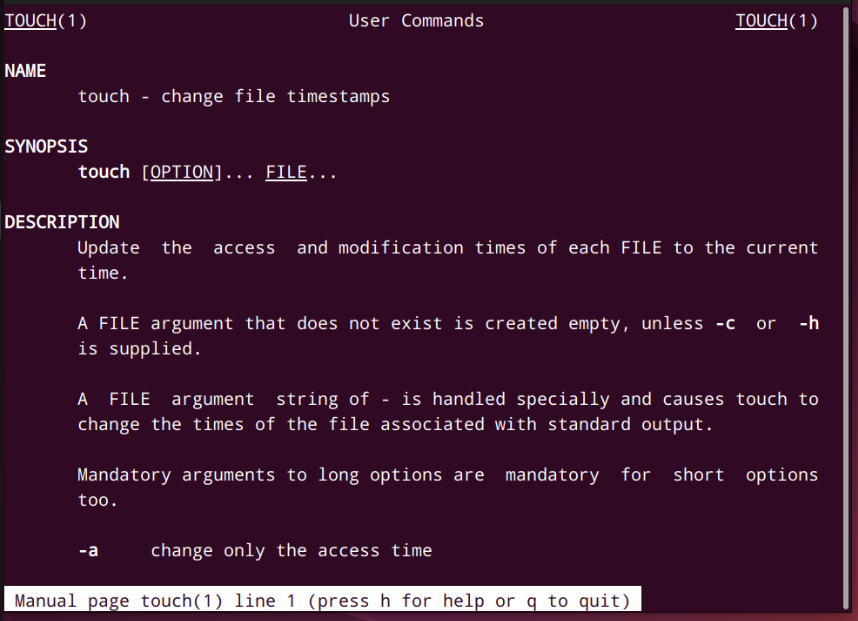
\includegraphics[width=0.5\linewidth]{figures/man_touch.png}
	\caption{如图所示为touch的man手册}
\end{figure}

\subsubsection{用 touch 在 missing 文件夹中新建一个叫 semester 的文件?}
\begin{lstlisting}
	touch /tmp/missing/semester
\end{lstlisting}
\begin{figure}[htbp]
	\centering
	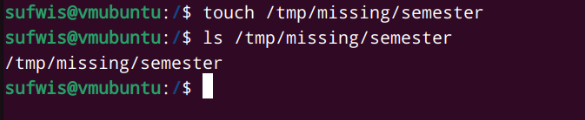
\includegraphics[width=0.7\linewidth]{figures/touch.png}
	\caption{如图,创建成功}
\end{figure}

\subsubsection{将以下内容一行一行地写入 semester 文件:}
\begin{verbatim}
#!/bin/sh
curl --head --silent https://missing.csail.mit.edu?
\end{verbatim}
\begin{lstlisting}
	use vim or echo
	use '' to include content if you choise echo
	Because for bash, the content within single quotes will not be processed
\end{lstlisting}
\begin{figure}[htbp]
	\centering
	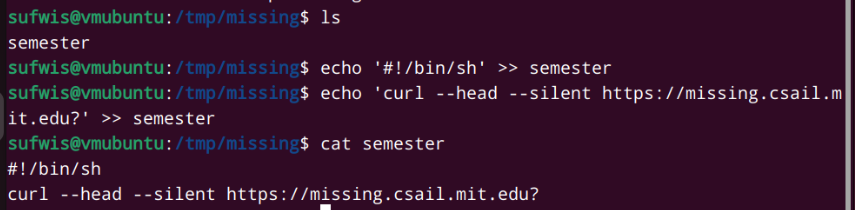
\includegraphics[width=0.7\linewidth]{figures/echo.png}
	\caption{如图,已经写入}
\end{figure}

\subsubsection{尝试执行这个文件。例如,将该脚本的路径(./semester)输入到您的 shell 中并回车?}
\begin{lstlisting}
	first, we could find the file does not have execution permission
	so, use chmod to add -x permission
	finally, execute it.
\end{lstlisting}
\begin{figure}[H]
	\centering
	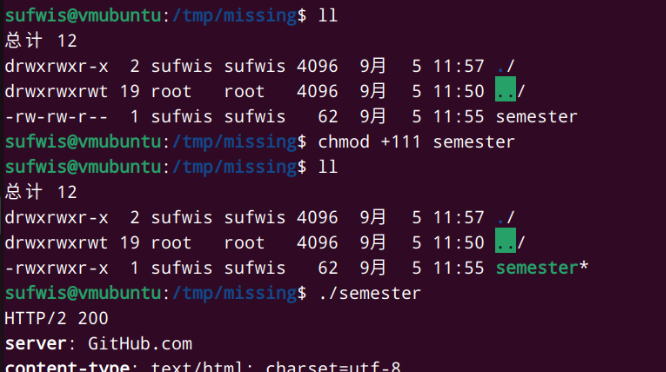
\includegraphics[width=0.7\linewidth]{figures/bash_se.png}
	\caption{结果如图,脚本执行后输出的部分内容被省略}
\end{figure}



\subsubsection{查看 chmod 的手册(例如,使用 man chmod 命令)?}
\begin{lstlisting}
	man chmod
	or
	chmod --help
\end{lstlisting}
\begin{figure}[htbp]
	\centering
	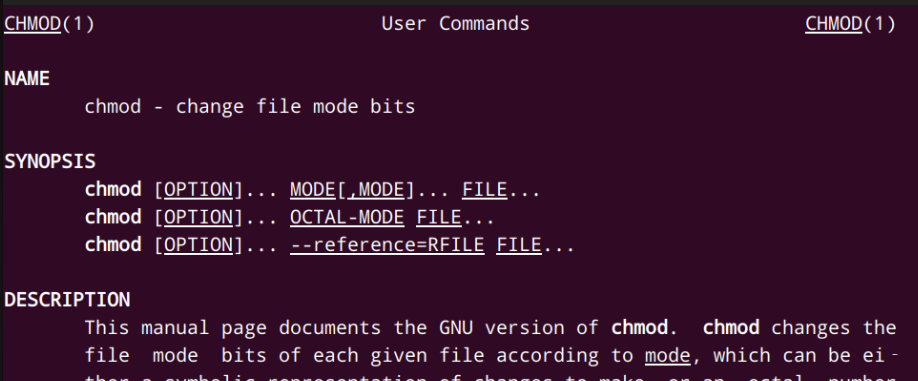
\includegraphics[width=0.7\linewidth]{figures/man_chmod.png}
	\caption{使用man chmod的结果}
\end{figure}
\textit{尽管man或者--help都能给出对应命令的解释,给出对应的参数,或者例子。但是如今,使用ai插件询问也是推荐的。}
\\

\subsubsection{使用 chmod 命令改变权限,使 ./semester 能够成功执行,不要使用 sh semester 来执行该程序。您的 shell 是如何知晓这个文件需要使用 sh 来解析呢?}
\hbox{\textbf{首先,如果要执行脚本,一般有两种方式:}}
\begin{enumerate}
	\item 解释器+脚本文件
	\item ./脚本文件
\end{enumerate}
第一种只会使用指定的解释器来执行脚本,且不需要脚本有可执行权限,第二种则会根据shebang执行,需求可执行权限。\\
因此,问题就明了了,先使用chmod为脚本提供可执行权限,然后./semester执行。\\
\begin{lstlisting}
	chmod +111 semester
	./semester
\end{lstlisting}
\begin{figure}[htbp]
	\centering
	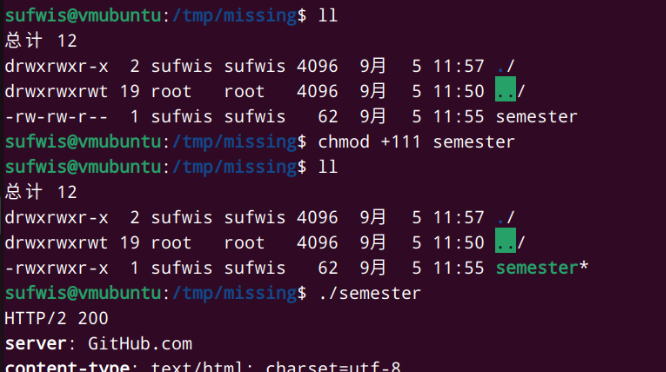
\includegraphics[width=0.7\linewidth]{figures/bash_se.png}
	\caption{已经执行过该脚本}
\end{figure}

\subsubsection{使用 \texttt{|} 和 \texttt{>} ,将 semester 文件输出的最后更改日期信息,写入主目录下的 last-modified.txt 的文件中}
\begin{lstlisting}
	touch ~/last-modified.txt # to make the file
	./semester | grep "last-modified" > ~/last-modified.txt
	# execute semester, use grep to get lines that include "last-modified", re-direct
\end{lstlisting}
\begin{figure}[H]
	\centering
	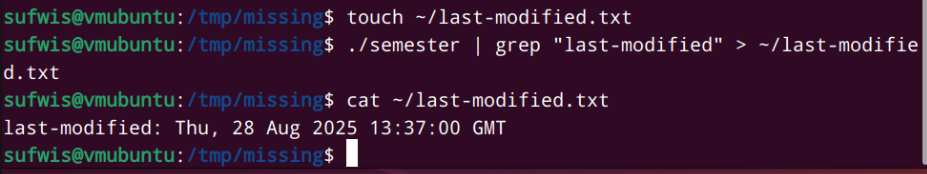
\includegraphics[width=0.7\linewidth]{figures/grep.png}
	\caption{如图}
\end{figure}

\subsubsection{写一段命令来从 /sys 中获取笔记本的电量信息?}
\noindent结论:\\
在物理 Linux 机器上,电量信息通常通过 sysfs 或 proc 文件系统提供,主要路径是:
\begin{verbatim}
	/sys/class/power_supply/。
\end{verbatim}
在这个目录下,你通常会看到像 BAT0(电池)或 AC(电源适配器)这样的文件夹。\\
在虚拟机中:\\
当你进入这个目录时,可能会有两种情况:
目录为空:虚拟机没有模拟电池设备,因此没有相关信息。
有一个 AC 设备:虚拟机通常会模拟一个始终连接电源适配器的状态,让你感觉它一直在通电运行。\\
\begin{lstlisting}
	cd /sys/class/power_supply/ACAD
	cat online
\end{lstlisting}
\begin{figure}[H]
	\centering
	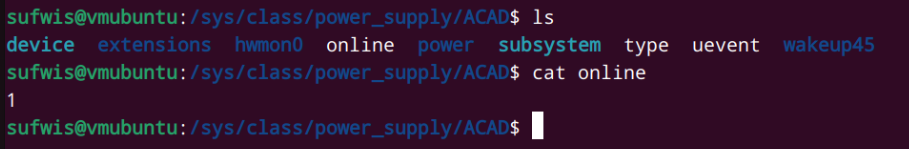
\includegraphics[width=0.7\linewidth]{figures/online.png}
	\caption{图中输出1,表明电源联通}
\end{figure}

\subsubsection{阅读 man ls ,然后使用 ls 命令进行如下操作?}
\begin{itemize}
	\item 所有文件(包括隐藏文件)
	\item 文件打印以人类可以理解的格式输出 (例如,使用 454M 而不是 454279954)
	\item 文件以最近修改顺序排序
	\item 以彩色文本显示输出结果
\end{itemize}
\begin{lstlisting}
	ls -a
	ls -h 
	ls -t
	ls --color=auto
\end{lstlisting}
\begin{figure}[H]
	\centering
	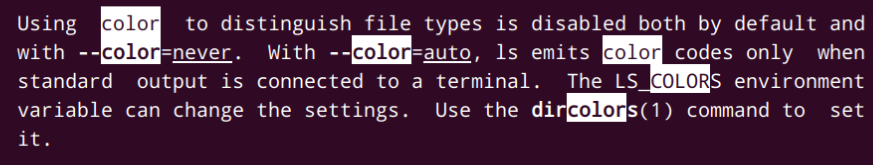
\includegraphics[width=0.7\linewidth]{figures/color.png}
	\caption{这是对--color参数的说明}
\end{figure}
\begin{figure}[H]
	\centering
	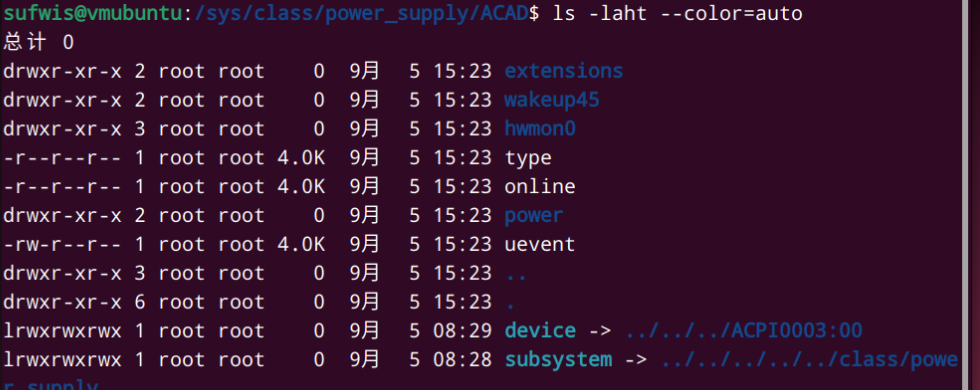
\includegraphics[width=0.7\linewidth]{figures/ls.png}
	\caption{ls综合结果}
\end{figure}

\subsection{bash脚本}
\subsubsection{编写两个 bash 函数 marco 和 polo 执行下面的操作}
每当你执行 marco 时,当前的工作目录应当以某种形式保存。
当执行 polo 时,无论现在处在什么目录下,都应当 cd 回到当时执行 marco 的目录。
为了方便 debug,你可以把代码写在单独的文件 marco.sh 中。
并通过 source marco.sh 命令,(重新)加载函数
涉及bash脚本语法和source加载脚本。\\
source能够更改当前shell环境,例如修改变量、函数等。\\
\begin{lstlisting}
	#!/usr/bin/bash
	marco_log_path="$HOME/logs/marco.log"
	marco(){
		echo "$(pwd)" > $marco_log_path
		echo "pwd saved; use polo to back"
	}
	polo(){
		cd "$(cat "$marco_log_path")"
	}
\end{lstlisting}
\begin{figure}[H]
	\centering
	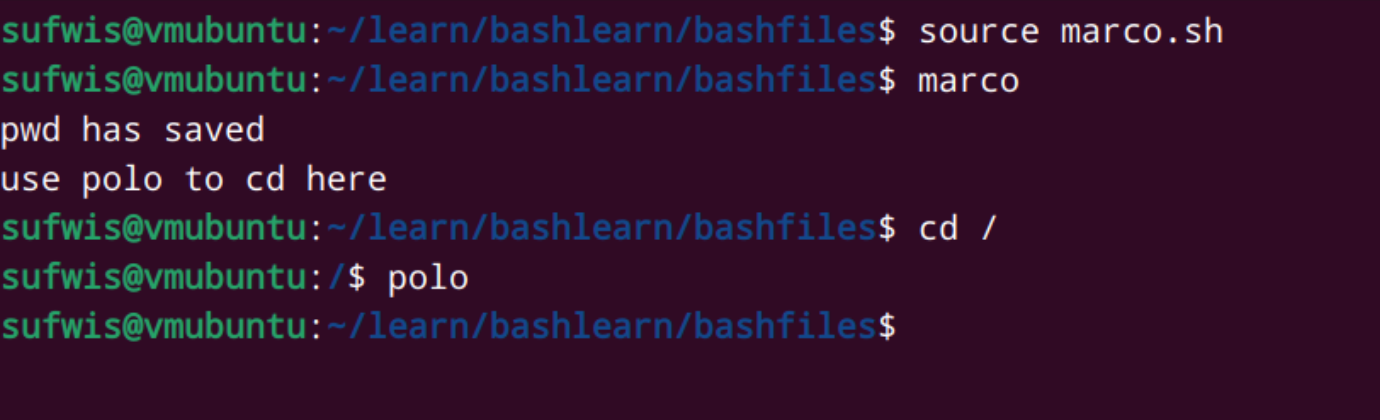
\includegraphics[width=0.7\linewidth]{figures/marco_polo.png}
	\caption{演示,代码略有不同}
\end{figure}

\subsubsection{编写一段 bash 脚本,完成以下任务?}
假设您有一个命令,它很少出错。
因此为了在出错时能够对其进行调试,
需要花费大量的时间重现错误并捕获输出。 
编写一段 bash 脚本,运行如下的脚本直到它出错,
将它的标准输出和标准错误流记录到文件,并在最后输出所有内容。 
加分项:报告脚本在失败前共运行了多少次。
\begin{lstlisting}
	#!/usr/bin/env bash

 	n=$(( RANDOM % 100 ))

 	if [[ n -eq 42 ]]; then
    	echo "Something went wrong"
    	>&2 echo "The error was using magic numbers"
    	exit 1
 	fi

 	echo "Everything went according to plan"
\end{lstlisting}
下面是一种解决方法:\\
\lstinputlisting{eq32.sh}
\begin{figure}[H]
	\centering
	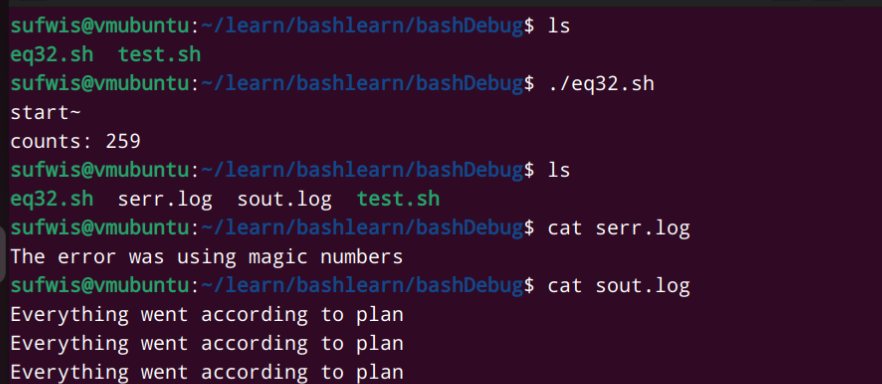
\includegraphics[width=0.7\linewidth]{figures/eq.png}
	\caption{结果如图}
\end{figure}

\subsubsection{我们已经知道,命令行可以从参数或标准输入接受输入。在用管道连接命令时,我们将标准输出和标准输入连接起来。任务:}
这里我们可以使用 xargs 命令,它可以使用标准输入中的内容作为参数。 
例如 ls | xargs rm 会删除当前目录中的所有文件。
\\
\indent 您的任务是编写一个命令,
它可以递归地查找文件夹中所有的 HTML 文件,
并将它们压缩成 zip 文件。
注意,即使文件名中包含空格,您的命令也应该能够正确执行。\\
\qquad -d 指定xargs的分隔符。
\begin{lstlisting}
	find . -name "*.html" -print0 | xargs -d '\0' tar cvfz all.tar.gz
\end{lstlisting}
\parbox{\linewidth}{
  \indent 使用-print0以null字符作为输出的分隔符,-d指定null字符,也可使用-0。
  倘若使用默认的空白分隔符,含有空格的文件两侧分别被当两个文件处理。%
}
\begin{figure}[H]
	\centering
	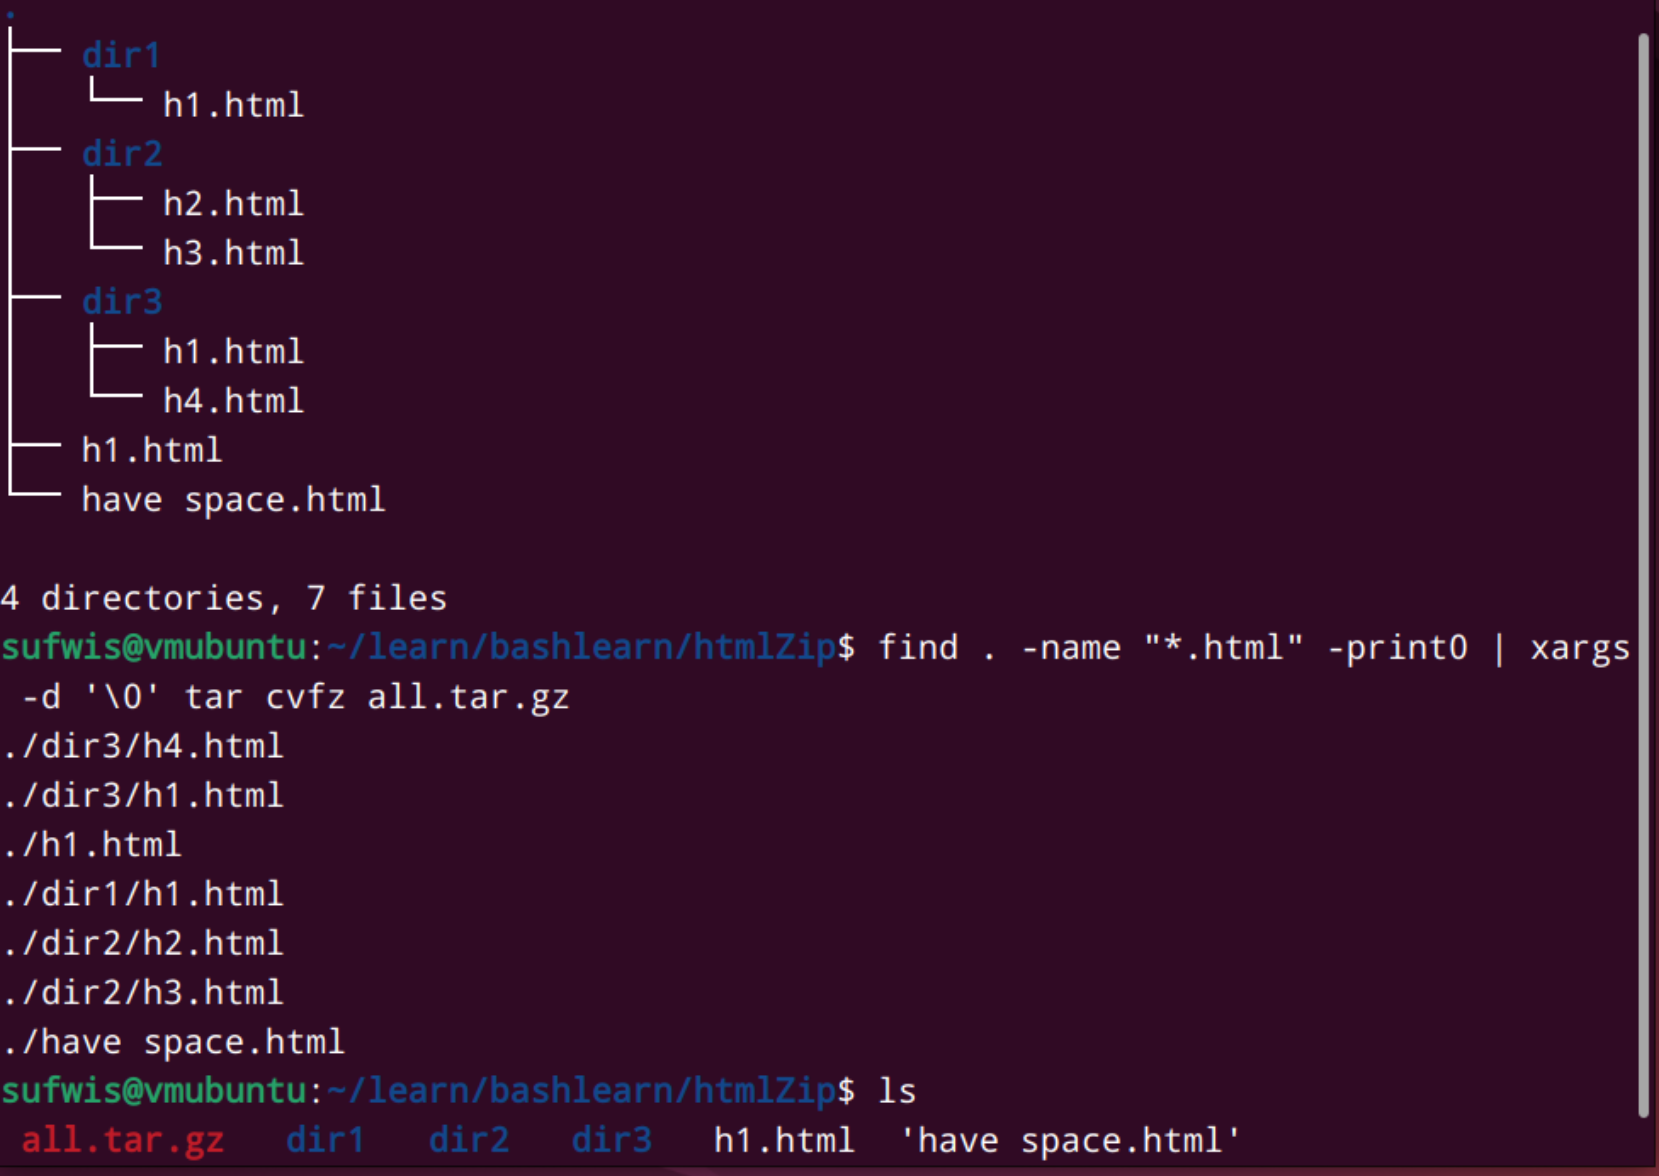
\includegraphics[width=0.7\linewidth]{figures/html.png}
	\caption{结果如图}
\end{figure}

\subsubsection{编写一个命令或脚本递归的查找文件夹中最近修改的文件。更通用的做法,你可以按照最近的修改时间列出文件吗?}
\begin{lstlisting}
	find . -mtime 0 -type f -print0 | xargs -0 ls -lt | head -5
	# man find to check -mtime -type -print0 or man head
\end{lstlisting}
\begin{figure}[H]
	\centering
	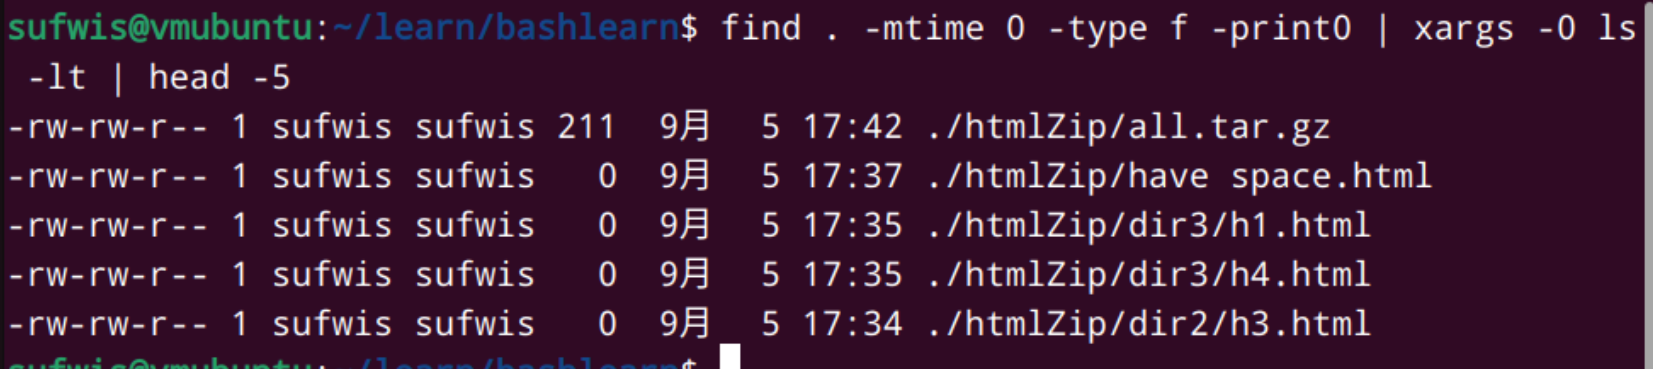
\includegraphics[width=0.7\linewidth]{figures/find_ls_t.png}
	\caption{结果如图,查找一天内按照修改顺序排序的前5个文件}
\end{figure}

\subsubsection{编写一个脚本,处理用户信息,演示字符串变量、数组和环境变量的使用?}
\begin{lstlisting}

\end{lstlisting}
\begin{figure}[H]
	\centering
	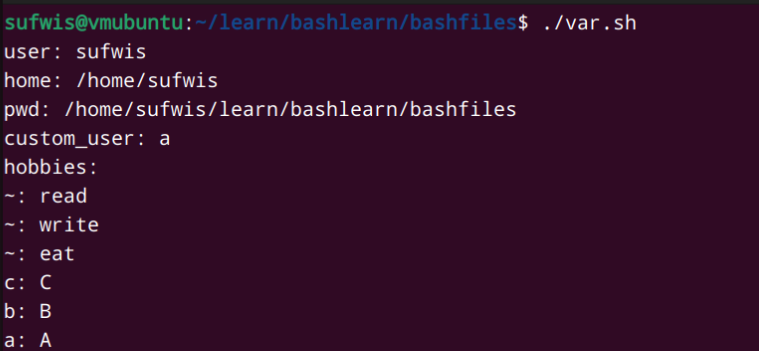
\includegraphics[width=0.7\linewidth]{figures/array.png}
	\caption{结果如图}
\end{figure}

\subsection{vim基础操作}
\subsubsection{完成 vimtutor?}
\begin{lstlisting}
	vimtutor
\end{lstlisting}
\begin{figure}[H]
	\centering
	
\includegraphics[width=0.7\linewidth]{figures/vimtutor.png}
	\caption{你将看到这样的画面,依照指示行动}
\end{figure}

\subsubsection{下载我们的 vimrc,然后把它保存到 ~/.vimrc。 通读这个注释详细的文件 (用 Vim!), 然后观察 Vim 在这个新的设置下看起来和使用起来有哪些细微的区别?}
这个vimrc文件已经放在本目录下。\\
\indent 将之重命名为.vimrc并放在加目录下,之后使用vim打开,你将看到:\\
\begin{figure}[H]
	\centering
	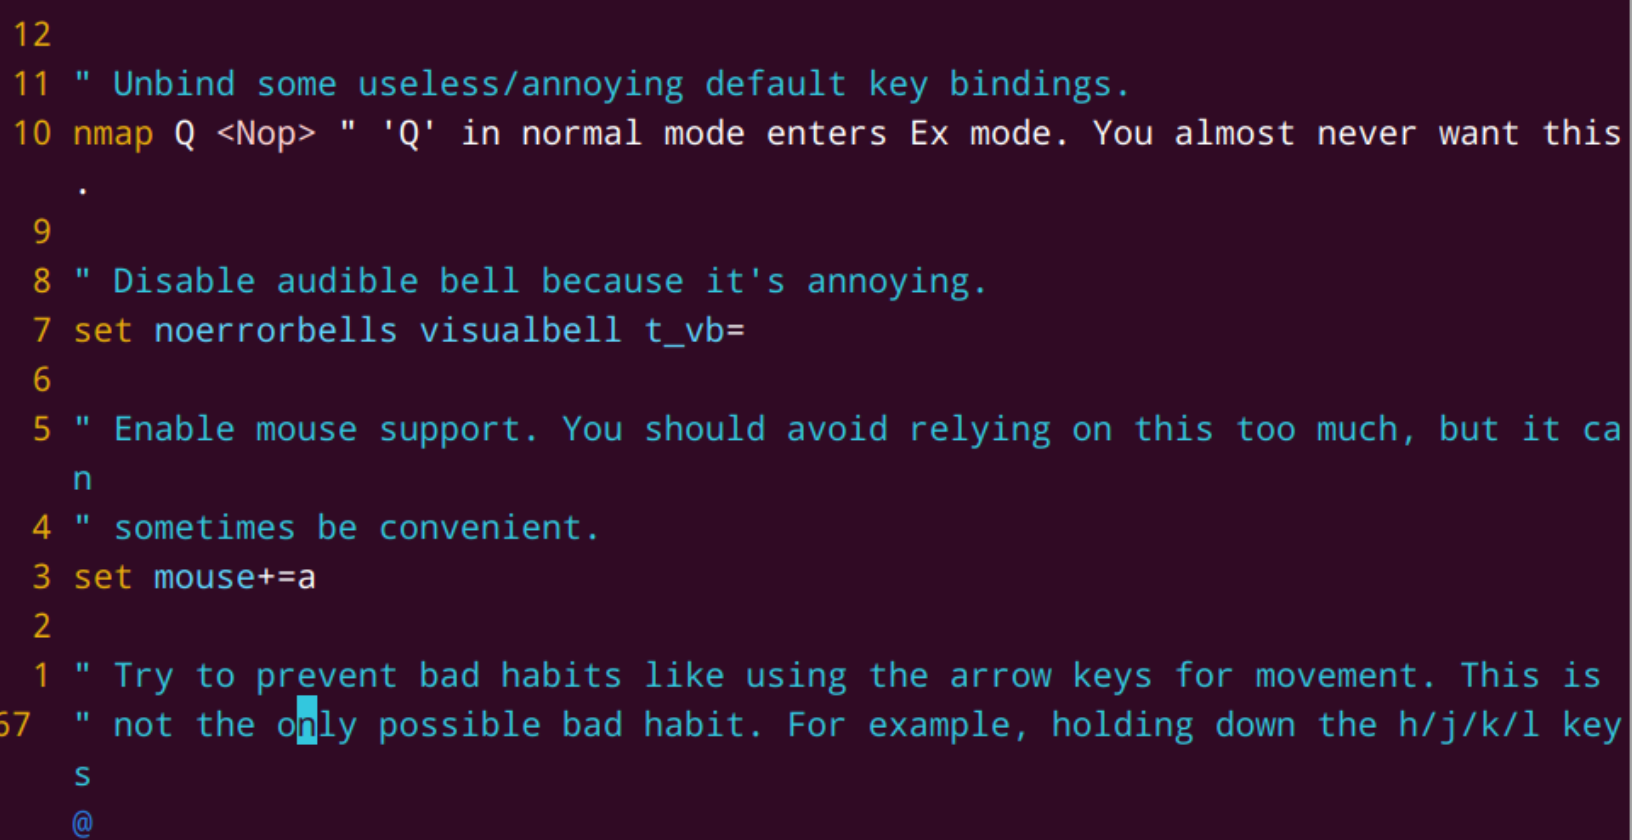
\includegraphics[width=0.7\linewidth]{figures/look_vimrc.png}
	\caption{参阅注释,尝试修改}
\end{figure}
\indent 例如set mouse+=a,a 代表 "all",意味着在所有模式(普通模式、插入模式、可视模式等)中都启用鼠标支持
没有这个设置时,Vim 通常只在普通模式和可视模式中支持部分鼠标功能。\\

\subsubsection{下载vim-plug?}
克隆vim-plug仓库,将plug.vim移动到~/.vim/autoload/下。之后修改 ~/.vimrc。\\
\indent 在call plug\verb|#|begin/end之间,使用Plug 'url'提供插件源,例如github、gitee仓库。之后source ./.vimrc
应用这个文件的更改,执行:PlugInstall下载,或者PlugUpdate更新。\\
\indent 如果想要删除插件,只需要删除Plug 'url'对应的那一行,然后:PlugClean即可。\\
\begin{lstlisting}
	 call plug#begin()
	 Plug 'preservim/NERDTree'
	 Plug 'wikitopian/hardmode'
	 .....
	 call plug#end()
\end{lstlisting}
\begin{figure}[H]
	\centering
	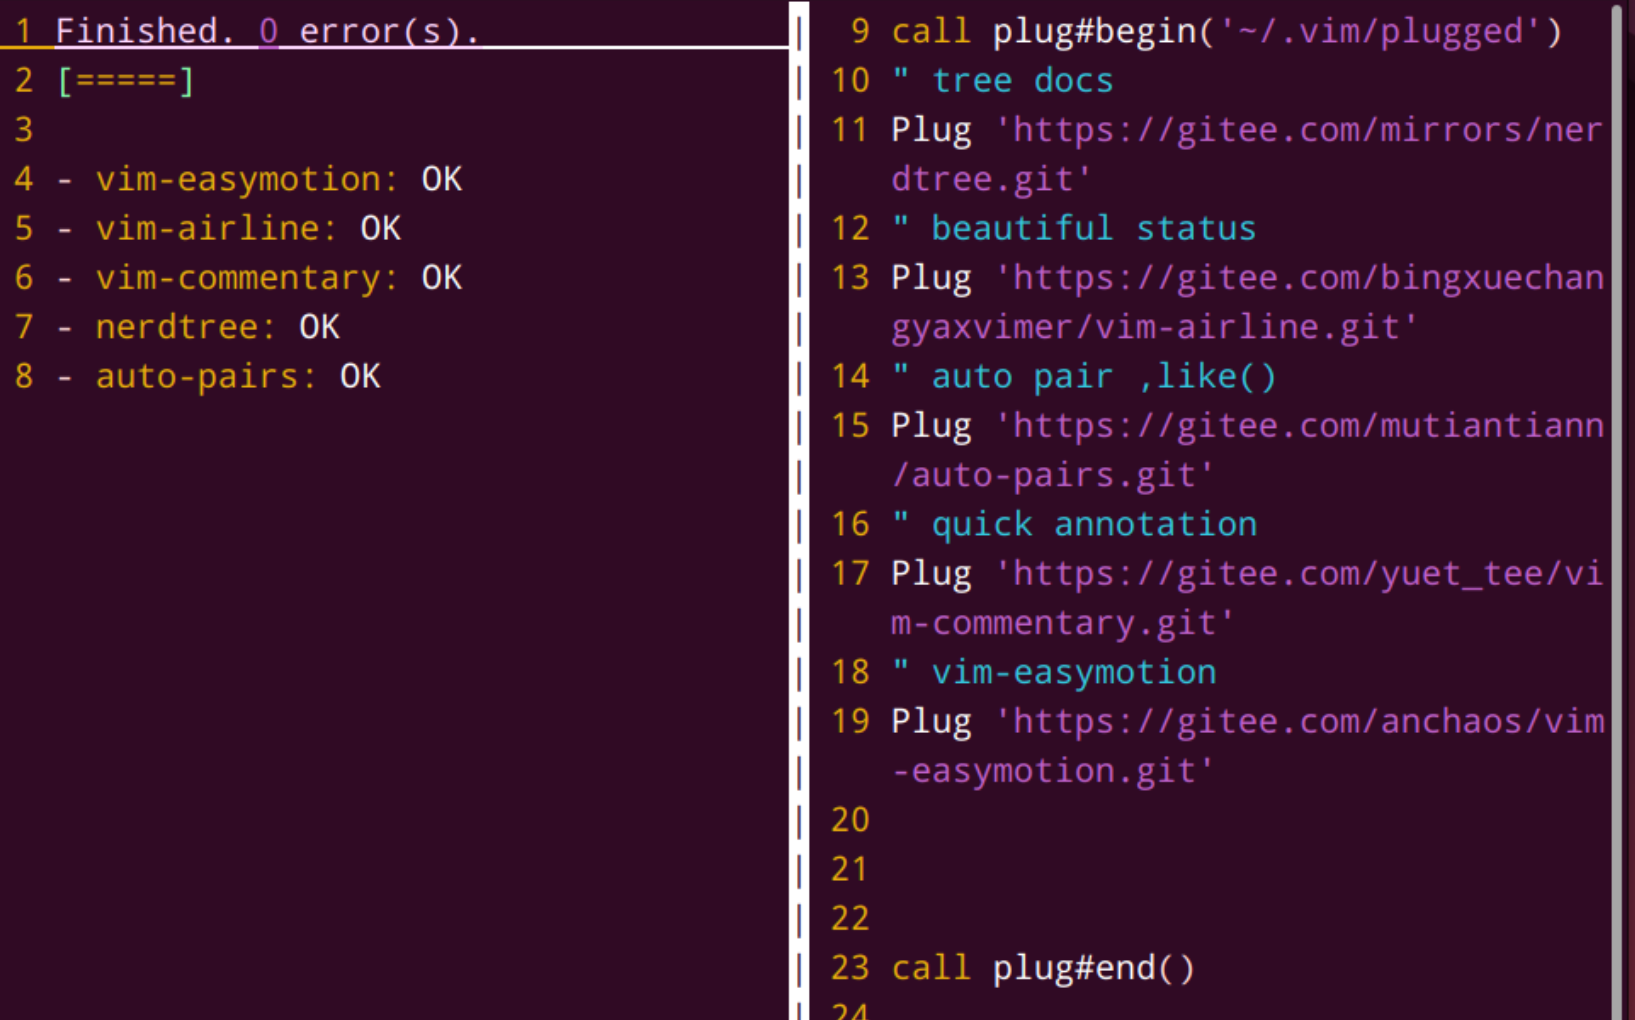
\includegraphics[width=0.7\linewidth]{figures/plug.png}
	\caption{如图,安装插件后可以通过:PlugStatus查看插件状态}
\end{figure}


\subsection{数据整理/正则表达式}
\subsubsection{统计 words 文件 (/usr/share/dict/words) 中包含至少三个 a 且不以 's 结尾的单词个数?}
\begin{lstlisting}
	# regular expr
	^([^a]*a){3}.*(?<!'s)$
	# if use grep
	cat /usr/share/dict/words | tr "[:upper:]" "[:lower:]" | grep -E "^([^a]*a){3}.*$" | grep -v "'s$" | wc -l
\end{lstlisting}
\begin{figure}[H]
	\centering
	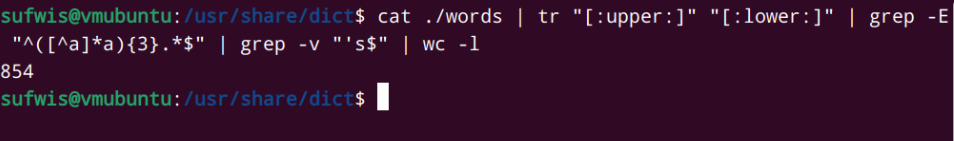
\includegraphics[width=0.7\linewidth]{figures/word_count.png}
	\caption{grep不支持零宽断言}
\end{figure}

\subsubsection{这些单词中,出现频率前三的末尾两个字母是什么?}
\begin{lstlisting}
	cat /usr/share/dict/words | tr "[:upper:]" "[:lower:]" | grep -E "^([^a]*a){3}.*$" | grep -v "'s$" |
	sed -E "s/.*([a-z]{2})$/\1/" | sort | uniq -c | sort | tail -n5
\end{lstlisting}
\begin{figure}[H]
	\centering
	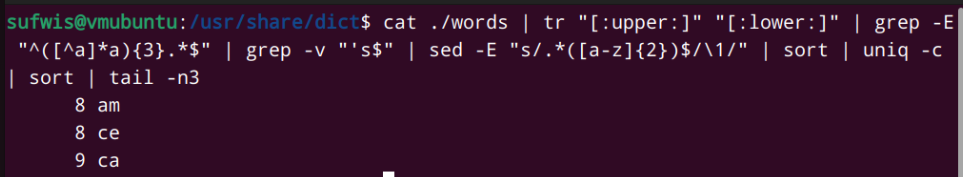
\includegraphics[width=0.7\linewidth]{figures/tail3.png}
	\caption{sed用于将单词简化为末尾两个字母,然后排序统计}
\end{figure}
\indent 通过tail -n10 查看,ah频次同样是8,所以仅仅使用tail -n3是不够的。\\



\section{实验感悟}
\indent shell/bash是计算机的一种文字接口,熟练使用能够缩短操作时间,不必使用鼠标,而是使用快捷的键盘。
如果仅仅是为使用,学习shell并不复杂。只需要浏览一些介绍shell操作的博客即可。\\
\indent 然而事实上并非如此简单,如同vim一样,它们提供很高的自由度,这需要使用者付出时间学习。
倘若想要更加顺手,或者自定义,更需要学习编写vim/shell本身的语言,例如使用vim script来编写插件。\\
\indent vim是一个熟手觉得好用,新手认为落后的编辑器。如果习惯于各种预先提供好的服务,那么选用现代IDE是不错的选择;
如果你认为IDE本身阻碍你的思考,让你的操作跟不上你的思维,那么vim更加便捷。\\
\indent 重要的是选择合适的,而非大众眼中最好的。因为合适的才是最好的。\\

\section{个人github/gitee账号}
\href{https://github.com/sufwis}{个人github账号}\\
\indent \href{https://github.com/sufwis/development-tools-learn.git}{对应仓库}

\section{参考资料}
\href{https://missing-semester-cn.github.io/}{计算机教育中缺失的一课}

\end{document}